\documentclass[11pt]{article}

\usepackage[T1]{fontenc}
\usepackage[
    left = 4cm,
    right = 4cm,
    top = 2cm,
    bottom = 3cm
]{geometry}
\usepackage{
    amsmath,
    amsfonts,
    bbm
}
% Fuentes bonitas
\usepackage{newpxtext,newpxmath}

\usepackage{enumerate}
% \usepackage{titling}
% \usepackage{tipa}
\usepackage[utf8]{inputenc}
\usepackage[spanish, mexico]{babel}
% \usepackage{csquotes}
% \usepackage{amsbsy}
\usepackage[spanish]{babel}
\usepackage{datetime}
% \usepackage{natbib}
% \usepackage{dsfont} 
% \usepackage{gensymb}
% \usepackage{textcomp}
\usepackage{flushend}
\usepackage{anyfontsize}

%%floor and ceilling
\usepackage{mathtools}
%% includegraphics command.
\usepackage{graphicx}
%% various useful mathematical symbols
\usepackage{amssymb}
%% extended theorem environments
% \usepackage{amsthm}


% Section size
\usepackage{sectsty}
    \sectionfont{\fontsize{13}{11}\selectfont}

\usepackage{float}
\usepackage{mathrsfs}

%Ref
\usepackage{hyperref}
\usepackage[spanish]{cleveref}

\usepackage[nottoc]{tocbibind}

%Figuras numeradas
\usepackage{chngcntr}
    \counterwithin{figure}{section}

% formato personalizado
\newdateformat{mydate}{\THEMONTH \THEDAY, \THEYEAR}
% definir fecha exacta
\newdate{hmw}{07}{09}{2019}

\usepackage{tcolorbox}

\usepackage{fancyhdr}

\newcounter{tarea}

\pagestyle{fancy}
    \fancyhf{}
    \rhead{\fecha}
    \lhead{\autor}
    \rfoot{\textit{\textbf{Página \thepage}}}


% ------- Conjuntos -------

\newcommand{\set}[1]{   % Descripción conjunto cualquiera (llaves)
    \left\{
        #1
    \right\}
}

    % Conjuntos de números

\newcommand{\N}{    % Números naturales
    \mathbb{N}
}
\newcommand{\Z}{    % Números enteros
    \mathbb{Z}
}
\newcommand{\Q}{    % Números racionales
    \mathbb{Q}
}
\newcommand{\I}{    % Números irracionales
    \mathbb{I}
}
\newcommand{\R}{    % Números reales
    \mathbb{R}
}
\newcommand{\C}{    % Números complejos
    \mathbb{C}
}
\newcommand{\F}{    % Campo arbitrario ?
    \mathbb{F}
}

    % Topología

\newcommand{\Fr}{
    \mathrm{Fr}\,
}

\newcommand{\cl}[1]{
    \overline{#1}
}
\newcommand{\interior}{
    \mathrm{int}\,
}

    % Conjuntos asociados a funciones

\newcommand{\im}[1]{    % Imagen de una función
    \mathrm{Im} \,
}
\newcommand{\dom}[1]{   % Dominio de una función
    \mathrm{Dom} \,
}

    % Conjuntos asociados a funciones de Álgebra Lineal

\newcommand{\kernel}[1]{   % Kérnel de una transformación lineal
    \mathrm{Ker} \,
}
\newcommand{\setspan}[1]{   % Espacio generado por un conjunto
    \mathrm{span} \,
}

% ------- Funciones -------

    % Normas

\providecommand{\abs}[1]{   % Valor absoluto
    \left\vert
        #1
    \right\vert
}
\providecommand{\norm}[1]{  % Norma
    \left\lVert
        #1
    \right\rVert
}
\providecommand{\prodint}[1]{   % Producto interior
    \left\langle
        #1
    \right\rangle
}

    % Probabilidad

\newcommand{\Esp}[1]{   % Esperanza matemática
    E
    \left[
        #1
    \right]
}
\newcommand{\Prob}[1]{  % Probabilidad
    P
    \left[
        #1
    \right]
}
\newcommand{\ind}[2]{   % Función indicadora / Función característica
    1_{#1}
    \left(
        #2
    \right)
}

    % dimensiones de Álgebra Lineal

\renewcommand{\dim}[2][]{   % Dimensión
    \mathrm{dim} \,
}
\newcommand{\rango}[1]{ % Rango (dimensión del espacio imagen)
    \mathrm{rango} \,
}
\newcommand{\nulidad}[1]{   % Nulidad (dimensión del kérnel)
    \mathrm{nulidad} \,
}

    % Números complejos
\newcommand{\repart}[1]{
    \mathrm{Re}
    \left(
        #1
    \right)
}
\newcommand{\impart}[1]{
    \mathrm{Im}
    \left(
        #1
    \right)
}

% ----- Mapeos -----

\newcommand{\To}{   % Flecha larga
    \longrightarrow
} 
\newcommand{\mTo}{ % Flecha larga con cola (manda a)
    \longmapsto
} 

% ----- Lógica -----

\newcommand{\ssi}{  % Si y solo si (<=>)
    \Leftrightarrow
}
\newcommand{\ent}{  % Entonces (=>)
    \Rightarrow
}
\newcommand{\Ent}{  % Entonces largo (==>)
    \Longrightarrow
}
\newcommand{\Ssi}{  % Si y solo si largo (<==>)
    \Longleftarrow
}

% ----- Letras especiales ------

\newcommand{\eps}{  % Épsilon bonita (siempre varépsilon)
    \varepsilon
}

\newcommand{\uphi}{
    \phi
}
\renewcommand{\phi}{
    \varphi
}

\newcommand{\titulo}{
    \textsc{
        \textcolor{tscolor}{\textbf{\tema.} Variable Compleja}
    }
}

\newcommand{\autor}{
    \textbf{Estudiante:} Juan Armando Parra Flores
}

\newcommand{\fecha}{
    \textbf{Fecha:} \today
}

% Definiciones de teoremas, definiciones...

% \newtheorem{axiom}{Axioma}
% \theoremstyle{definition}
% \newtheorem{definition}{Definición}[section]
% \newtheorem{theorem}{Teorema}[section]
% \newtheorem{lemma}{Lema}[section]
% \newtheorem{corollary}[theorem]{Corolario}
% \newtheorem{proposition}[theorem]{Proposición}
% \theoremstyle{remark}
% \newtheorem*{note}{\bfseries Nota}
% 
% \crefname{definition}{Definición}{Definiciones}
% \crefname{axiom}{Axioma}{Axiomas}
% \crefname{theorem}{Teorema}{Teoremas}
% \crefname{lemma}{Lema}{Lemas}
% \crefname{corollary}{Corolario}{Corolarios}
% \crefname{proposition}{Proposición}{Proposiciones}
% \crefname{section}{Sección}{Secciones}
% 
% \newenvironment{solution}{\begin{proof}[Solución]}{\end{proof}}
% \renewcommand{\qedsymbol}{$\blacksquare$}
% 
% \newcommand{\QED}{$\hfill\blacksquare$} % Pone el cuadrito negro hasta el final de la línea
% \newcommand{\EndSol}{$\hfill\square$} % Cuadrito blanco al final al final de la línea

\newenvironment{proof}[1][\textbf{\textit{Demostración}}]{
     \par\medskip\noindent \textcolor[rgb]{0.6,0,0.3}{#1.}
     \rmfamily
}{
    % \par
    % $\hfill\textcolor[rgb]{0.2,0,0.6}{\textbf{QED}}$\\
    $\hfill\textcolor[rgb]{0.6,0,0.3}{\blacksquare}$\\
}

\newenvironment{solution}[1][\textbf{\textit{Solución}}]{
     \par\medskip\noindent \textcolor[rgb]{0.6,0,0.3}{#1.}
     \rmfamily
}{
    \par
    % $\hfill\textcolor[rgb]{0.2,0,0.6}{\textbf{S}}$\\
    $\hfill\textcolor[rgb]{0.6,0,0.3}{\square}$\\
}

\renewenvironment{boxed} % [1][]
{
    \begin{center}
    \begin{tabular}{|p{0.7\textwidth}|}
    \hline
}{ 
    \\
    \hline
    \end{tabular} 
    \end{center}
}

\newcounter{problem}
\newenvironment{problem}[1][\theproblem]{
    \begin{tcolorbox}[colback=purple!20,colframe=purple!50]
        \refstepcounter{problem}
        % \par\medskip
        % \noindent 
        % \color[rgb]{0.1,0.1,0.1}
        % \color[rgb]{0.1,0,0.5}
        \textbf{Problema~#1.}
        \rmfamily
}{
    \end{tcolorbox}
    \medskip
}


\title{
    \textsc{
        \textbf{Tarea 2.} Cálculo Diferencial e Integral IV
    }
}

\author{
    \textbf{Estudiante:} Juan Armando Parra Flores
}
\date{
    \textbf{Fecha:} \today
}

\begin{document}

    \maketitle

        % ========================== EJERCICIOS ========================== 
    \section*{Ejercicio 1}
    \begin{itemize}
        \item[3-26.]   
            Sea \( f: [a,b] \to \R \) integrable y no negativa, y sea \( A_f = \set{( x,y ) : 
a\leq x \leq b \text{ y } 0\leq y \leq f(x) } \). Demuestra que \( A_f \) es medible de
Jordan, y tiene área \( \integral{a}{b}{f} \).
\begin{proof}
    La frontera de $A_f$ es
    \begin{align*}
        \partial A_f 
        &=
        \set{
            (a,y)
            :
            0\leq y \leq f(a)
        }
        \cup
        \set{
            (b,y)
            :
            0\leq y \leq f(b)
        }
        \\
        &\quad
        \cup
        \set{
            (x,f(x)):
            a\leq x \leq b
        }
        \cup
        \set{(x,0):a\leq x\leq b}.
    \end{align*}
    Sea \( \eps >0 \), si $0 < \delta < \frac{\eps}{2f(a)+4} $, el rectángulo \( R= [ a - \delta , 
    a + \delta ] \times \left[ - 1, f(a) + 1 \right]   \) contiene al conjunto
    \( 
        \set{
            (a,y)
            :
            0\leq y \leq f(a)
        }
    \) y tiene volumen \( \mathrm{vol}(R)=
    2\delta ( f(a) + 2) = \delta (2f(a)+4)< \eps \). Por lo tanto
    \( 
        \set{
            (a,y)
            :
            0\leq y \leq f(a)
        }
    \) tiene contenido cero. 

    De forma similar, tomando \( \delta < \frac{\eps}{2f(b)+4} \) el conjunto
    \( 
        \set{
            (b,y)
            :
            0\leq y \leq f(b)
        }
    \), está contenido en el rectángulo \( \left[ b-\delta, b + \delta \right] \times
    \left[ -1,f(b)+1 \right]\), con volumen menor que \( \eps \). Así que este
    conjunto también 
    tiene contenido 0.

    El conjunto \( \set{(x,f(x)):a\leq x \leq b} \) es la gráfica de una función integrable, 
    por 
    cual tiene contenido 0. 
    La función constante 0 también es integrable, por lo que su gráfica 
    \( \set{(x,0):a\leq x \leq b }\) tiene contenido 0.

    Elc onjunto 
    \( \partial A_f \) es la unión finita de conjuntos de contenido 0. Por lo tanto tiene 
    contenido cero y \( A_f \) es medible de Jordan con área
    \begin{align*}
        \mathrm{area}(A_f)
        &=
        \int_{A_f}
        1
        =
        \int_{[a,b]\times [0, \max{f}]}
        \chi_{A_f}\\
        &=
        \int_{a}^b
        \int_{0}^{\max f}
        \chi_{A_f}(x,y) dy\,dx\\
        &=
        \int_{a}^b
        \left(
        \int_{0}^{f(x)}
        \chi_{A_f}(x,y) 
        dy
        +
        \int_{f(x)}^{\max f}
        \chi_{A_f}(x,y)
        dy\,
        \right)
        dx.
    \end{align*}
    Pero siempre que \( x\in [a,b] \) 
    cuando $y> f(x)$, $\chi_{A_f}(x,y)=0$, y su integral es 0, y cuando 
    \( 0 \leq y \leq f(x) \), \( \chi_{A_f}(x,y)=1 \). Por lo tanto
    \begin{align*}
        \mathrm{area}(A_f)
        &=
        \int_{a}^b
        \int_{0}^{f(x)}
        \chi_{A_f}(x,y) 
        dy
        \,
        dx\\
        &=
        \int_{a}^b
        \int_{0}^{f(x)}
        1\,
        dy
        \,
        dx\\
        &=
        \int_a^b
        x
        {\rvert_0^{f(x)}}
        dx\\
        &=
        \int_a^b
        f(x)
        \,
        dx.
    \end{align*}
\end{proof}

        \item[3-32.]   
            Sea \( f:[a,b]\times [ c,d ] \to \R \) continua, y subponga que 
\( D_2f \) es continua. Sea \( F(y) = \int_a^b f(x,y)dx \). Demuestre la
regla de Leibniz: \( F'(y) = \int_a^b D_2 f(x,y)dx \). 

\textit{Hint:} 
\( F(y) = \int_a^b f(x,y)dx = \int_a^b \left( \int_c^y D_2f ( x,t ) dt
+ f(x,c)\right) dx \). (La prueba mostrará que la continuidad de 
\( D_2f \) podría remplazarse por una hipótesis considerablemente más debil).
\begin{proof}
    Por el teorema fundamental del cálculo, para cada $x\in[a,b]$ 
    existe una constante \( K_x\in\R \),
    tal que como función de $y$, \( f(x,y) = \int_c^y D_2f(x,t)\,dt + K_k \). Tomando $y=c$
    podemos ver que $K+0=f(x,c)$. Por lo tanto 
    \( f(x,y)=\int_c^y D_2f(x,t)\,dt + f(x,c) \).
    Entonces
    \begin{align*}
        F(y)
        &=
        \int_a^b
        \left( 
            \int_c^y
            D_2f(x,t)\, dt
            +f(x,c)
        \right) \,dx\\
        &=
        \int_a^b
            \int_c^y
            D_2f(x,t)
            \, dt
        \, dx
        +
        \int_a^b
            f(x,c)
        \,dx.
    \end{align*}
    Observemos que la $y$ es fija y no está en función de $t$ ni de $x$. Por lo tanto 
    $F(y)$ está definida por el rectángulo de integración \( [ a,b ] \times [ c,y ] \), por
    lo que el teorema de Foubini nos permite intercambiar el orden de integración y ver que 
    \begin{align*}
        F(y)
        &=
        \int_c^y
            \int_a^b
            D_2f(x,t)
            \, dx
        \,dt
        +
        \int_a^b
        f(x,c)
        \,dx.
    \end{align*}
    Por el teorema fundamental del cálculo, al derivar con respecto a la variable $y$, obtenemos
    \begin{align*}
        F'(y)
        &=
        \int_a^b D_2f(x,t)\,dt,
    \end{align*}
    que era lo que queríamos probar.
\end{proof}

        \item[3-33.]   
            Si \( f : [ a,b ] \times [ c,d ] \to \R \) es continuoa y \( D_2f \) es continua,
defina \( F(x,y) = \int_a^x f(t,y)dt \).
\begin{enumerate}[(a)]
    \item
        Encuentra \( D_1F \) y \( D_2F \).
        \begin{solution}
            Por el ejercicio anterior, si se fija $x$, 
            \[
                D_2 F(x,y)
                =
                \int_a^x D_2 f(t,y)\, dt.
            \]
            Por el teorema fundamental del cálculo, cuando $y$ está fija, 
            \begin{align*}
                D_1 F(x,y)
                &=
                \frac{\partial}{\partial x} 
                \int_a^x
                f(t,y)\, dt\\
                &=
                f(x,y).
            \end{align*}
        \end{solution}
    \item
        Si \( G(x) = \int_a^{g(x)} f(t,x)dt \), encuentra \( G'(x) \).
        \begin{solution}
            Sea $F(x,y)=\int_a^x f(t,y)\,dt$, y notemos que 
            \( F(g(x),x)=G(x) \). Por la regla de la cadena en espacios más grandes, 
            \begin{align*}
                G'(t)
                &=
                D_1F(g(x),x)g'(x)
                +
                D_2F(g(x),x)\\
                &=
                f(g(x),x)g'(x)
                +
                \int_a^{g(x)}
                D_2f(t,x)\,dt.
            \end{align*}
            Este último paso se usa aplicando el inciso (a).
        \end{solution}
\end{enumerate}

    \end{itemize}
    \section*{Ejercicio 2}
    \begin{itemize}
        \item[6.]
            Usando el principio de Cavalieri, calcula el volumen de la estructura mostrada
en la figura; cada sección de cruce es un rectángulo de longitud 5 y ancho 3.
\begin{figure}[H]
    \begin{center}
        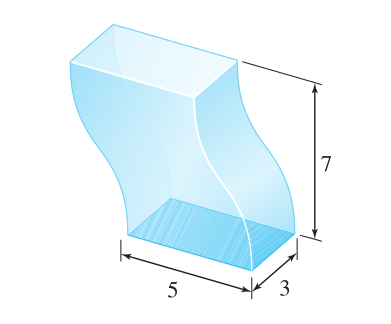
\includegraphics[width=0.3\textwidth]{img/Ej2/ej6.png}
    \end{center}
\end{figure}
\begin{solution}
    Sea $A(h)$, el área de la sección de cruce rectangular en la altura $h$. El principio 
    de Cavalieri dice que 
    el volumen de esta estructura es
    \begin{align*}
        \int_{0}^7 A(h) \, dh
        &=
        \int_{0}^7 5\cdot 3 \, dh\\
        &=
        15 \int_0^7 \, dh\\
        &=
        15 (7-0)=105.
    \end{align*}
\end{solution}

        \item[7.]
            Un leñador corta una pieza en forma de cuña $W$ de un árbol cilíndrico de radio $r$
obtenido de hacer dos cortes de sierra en el centro del árbol, uno horizontal
y otro en un ángulo $\theta$. Calcula el volumen de la cuña $W$ usando el 
principio de Cavalieri. 
Véase la figura
\begin{figure}[H]
    \begin{center}
        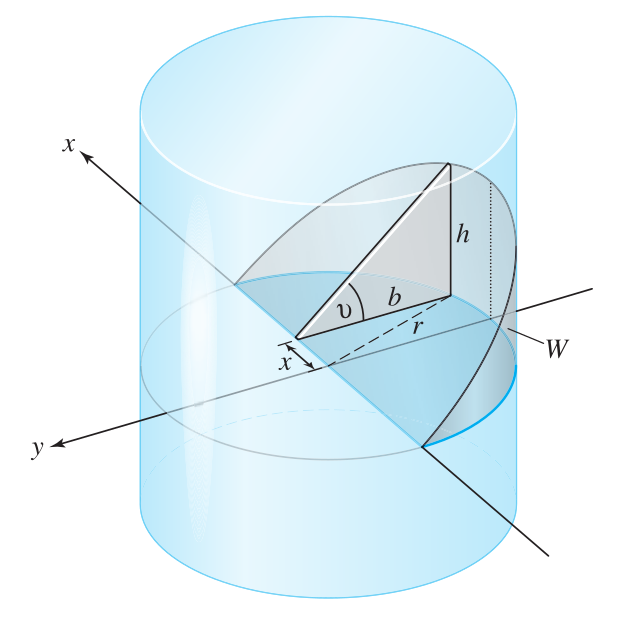
\includegraphics[width=0.3\textwidth]{img/Ej2/ej7.png}
    \end{center}
\end{figure}
\begin{solution}
    Como lo muestra la figura, podemos pensar en las secciones triangulares paralelas que dependen
    de $x$, que es la distancia de la punta de la sección al centr del círculo.
    Por otro lado, podemos observar un triángulo rectángulo formado por los de 
    longitud $x$, $r$ y $b$. Por lo tanto 
    \[
        b=\sqrt{r^2-x^2}.
    \]
    Así que podemos ver, 
    por la definición de tangente, que $h=b\tan \theta=\sqrt{r^2-x^2}\tan \theta$.
    Entonces el área de cada triángulo es 
    \[
        T(x)
        =
        \frac{1}{2} 
        \left(\sqrt{r^2-x^2}\right)
        \left( \sqrt{r^2-x^2}\tan \theta \right).
    \]
    De esta manera, por el principio de Cavalieri el volumen de la cuña es 
    \begin{align*}
        \mathrm{vol}(W)
        &=
        \int_{-r}^{r}
        T(x)
        \, dx
        =
        \int_{-r}^{r}
        \frac{\tan\theta}{2} (r^2-x^2)
        \, dx
        \\
        &=
        \tan\theta
        \int_{0}^{r}
        (r^2-x^2)
        \, dx,\quad\text{por la paridad del integrando,}\\
        &=
        \tan \theta
        \int_{0}^r
        r^2\, dx
        -\tan\theta
        \int_0^r
        x^2\, dx\\
        &=
        r^3\tan\theta-\tan\theta \frac{r^3}{3} = \frac{2 r^3 \tan \theta}{3}.
    \end{align*}
\end{solution}

        \item[8 b).]
            Demuestra que el volumen de la región obtenida 
por rotar la región debajo de la gráfica de la parábola
$y=-x^2+2x+3$, $-1\leq x\leq 3$, al rededor del eje
$x$ es $512 \frac{\pi}{15}$. 
Véase la figura
\begin{figure}[H]
    \begin{center}
        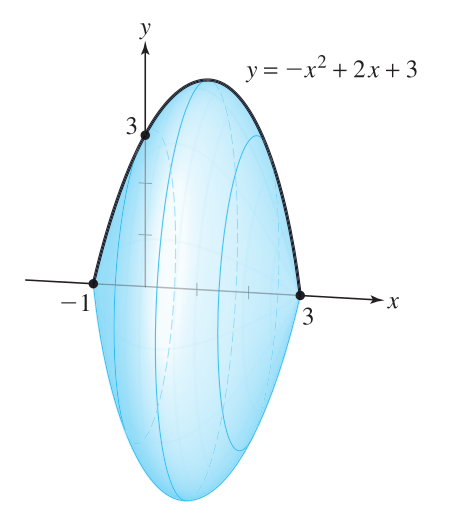
\includegraphics[width=0.3\textwidth]{img/Ej2/ej8b.png}
    \end{center}
\end{figure}
\begin{solution}
    Las secciones de corte con planos paralelos al plano \( yz \) son círculos de 
    radio \( y \), con área \( \pi y^2(x) = \pi (-x^2+2x+ 3)^2 \). Por el principio de 
    Cavalieri, el volumen de la región es 
    \begin{align*}
        \int_{-1}^3
        \pi y^2(x)
        \, dx
        &=
        \pi
        \int_{-1}^3
        (-x^2+2x+3)^2
        \, dx\\
        &=
        \pi
        \int_{-1}^3
        x^4-4x^3-2x^2+12x+9
        \,dx\\
        &=
        \left.
        \pi
        \left[ \frac{x^5}{5} -x^4- \frac{2x^3}{3} +6x^2+9x \right] \right|_{-1}^3\\
        &=
        \frac{512}{15} \pi
    \end{align*}
\end{solution}

        \item[14.]
            Encuentra el volumen acotado por la gráfica de 
$f(x,y)=1+2x+3y$, el rectángulo 
$[1,2]\times [0,1]$, y los cuatro lados verticales del rectángulo 
$R$
como en la figura
\begin{figure}[H]
    \begin{center}
        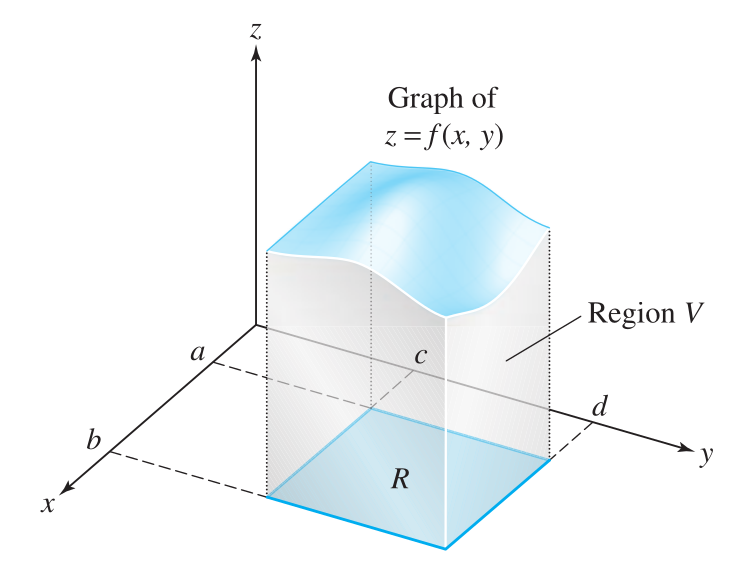
\includegraphics[width=0.3\textwidth]{img/Ej2/ej14.png}
    \end{center}
\end{figure}
\begin{solution}
%     La gráfica de esta función es un plano por lo que su máximo está ubicado en la frontera
%     del dominio de $f$. Pero por la fórmula de $f$ es fácil ver que mientras más grande sea 
%     $x$ y más grande sea $y$ se alcanzará el máximo en el punto
%     en el punto $(2,1)$, dejando como tal máximo a \( f(2,1)=8 \).
%     Igualmente podemos deducir que el mínimo de \( f \) está en \( (1,0) \) con su valor de 
%     \( f(1,0)=3>0 \). 
% 
    Podemos ver las intersecciones de los planos paralelos al plano \( yz \) y dependiendo 
    del valor de $x$, podemos ver que estos tienen
    área
    \[ \int_{0}^1 1+2x+3y \, dy = \left. \left[ y+2xy+3 \frac{y^2}{2} \right] \right\rvert_0^1 =
    \frac{5}{2} +2x.\] 
    Luego, por Cavalieri,  el volumen de la figura entera es 
    \begin{align*}
        \int_1^2
        \frac{5}{2} +2x \, dx
        &=
        \left.
        \left[ \frac{5}{2} x + x^2 \right] \right\rvert_1^2\\
        &=
        5+4- \frac{5}{2} - 1\\
        &=
        \frac{11}{2}.
    \end{align*}
\end{solution}

    \end{itemize}
    \section*{Eercicio 3}
    \begin{itemize}
        \item[1 d).]
            Calcula la siguiente integral si \(R =  [0,1]\times [ 0,1 ] \).
\[
    \iint_R\ln \left[ ( x+1 ) ( y+1 ) \right] dA.
\]
\begin{solution}
    Por el el Teorema de Foubini y la ley del logaritmo de un producto, 
    la integral anterior es igual a 
    \begin{align*}
        \int_{0}^1
        \int_0^1
        \ln(x+1)
        +\ln(y+1)
        \,dy
        \,dx.
    \end{align*}
    El integrando es 
    \begin{align*}
        \int_0^1\ln(x+1)\,dy+\int_0^1\ln(y+1)\,dy 
        &=
        y \left.
        \ln(x+1)+(y+1)(\ln(y+1)-1)\right
        \rvert_0^1\\
        &=
        \ln(x+1)
        +
        2(\ln(2)-1)
        +1\\
        &=
        \ln(x+1)
        +
        2\ln(2)
        -1.
    \end{align*}
    Entonces la integral anterior es
    \begin{align*}
        \int_0^1
        \ln(x+1)
        +2\ln(2)
        -1
        \, dx
        &=
        (x+1)(\ln(x+1)-1)
        +2\ln(2)x
        -x\rvert_0^1\\
        &=
        2(\ln(2)-1)
        +2\ln(2)-1
        -1(-1)\\
        &=
        4\ln(2)-2.
    \end{align*}
\end{solution}


        \item[4.]
            Calcula sobre la región \( R \):
\[
    \iint\limits_R \frac{y}{1+x^2} dydx,\quad R:[0,2]\times \left[ -1,1 \right].
\]
\begin{solution}
    \begin{align*}
        \int_{0}^2
        \int_{-1}^1
        \frac{y}{1+x^2} \,dy\,dx
        &=
        \int_0^2
        \frac{1}{1+x^2} 
        \int_{-1}^1
        y\,dy
        \,dx\\
        &=
        \int_0^2
        \frac{0}{1+x^2} \,dx,
        \quad\text{ya que $f(y)=y$ es impar,}\\
        &=
        0.
    \end{align*}
\end{solution}

        \item[5.]
            \begin{proof}
    
\end{proof}

        \item[10.]
            Calcula el volumen del sólido acotado por la superficie \( z=\sin y \), los
planos \( x=1 \), \( x=0 \), \( y=0 \) \( y= \frac{\pi}{2} \), y el plano \( xy \).
\begin{solution}
    La gráfica de este sólido luce más o menos como
    \begin{figure}[H]
        \begin{center}
            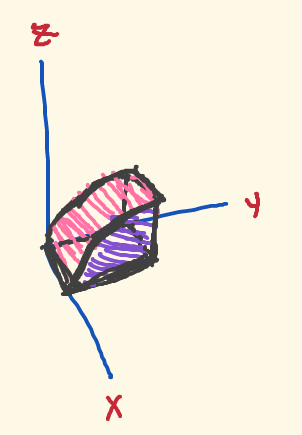
\includegraphics[width=0.3\textwidth]{img/Ej3/ej10.png}
        \end{center}
    \end{figure}
    Este volumen se puede calcular con el principio de Cavalieri con las secciones transversales
    \[
        C_x=\set{(x,y,z):0 \leq y\leq \frac{\pi}{2},0\leq z\leq \sin y},
    \]
    donde $0\leq x\leq 1$. Es decir, las intersecciones entre el sólido y los planos paralelos al 
    plano \( yz \).
    Por lo tanto el volumen de esta figura es 
    \begin{align*}
        \int_0^1
        \int_0^{\frac{\pi}{2}}
        \sin y
        \,dy
        \,dx
        &=
        \int_0^1
        -\cos \left( \frac{\pi}{2} \right)+
        \cos(0)
        \,dx\\
        &=
        \int_0^1 1 \, dx
        \\
        &=
        1
    \end{align*}
\end{solution}

    \end{itemize}
    % ======================== FIN DE DOCUMENTO ======================

\end{document}
